\documentclass[8pt,b5paper,tombo,openany]{jsbook}

\usepackage[dvipdfmx]{graphicx}
\usepackage{listings}
\usepackage{inconsolata}
\usepackage{url}
\usepackage{floatflt}
\usepackage{wrapfig}

\lstset{basicstyle={\small\ttfamily}}
\lstset{frame=single}
\lstset{breaklines=true}

\renewcommand{\kanjifamilydefault}{\gtdefault}
\renewcommand{\familydefault}{\sfdefault}

%%%% toc
% toc format
%\usepackage{tocloft}
% toc
\usepackage{minitoc}
\usepackage{titletoc}
\usepackage[]{titlesec}
\usepackage{tikz}
\usetikzlibrary{shadows.blur}

%\cftsetindents{chapter}{0.1in}{0.5in}
%\cftsetindents{section}{-0.25in}{0.5in}
%\cftsetindents{subsection}{-0.2in}{0.5in}

\definecolor{yourcolor}{HTML}{008bb2}

\colorlet{chpnumbercolor}{black}
\makeatletter
\let\oldl@chapter\l@chapter
\def\l@chapter#1#2{\oldl@chapter{#1}{\textcolor{chpnumbercolor}{#2}}}

\let\old@dottedcontentsline\@dottedtocline
\def\@dottedtocline#1#2#3#4#5{%
  \old@dottedcontentsline{#1}{#2}{#3}{#4}{{\textcolor{chpnumbercolor}{#5}}}}
\makeatother

\titleformat{\chapter}[display]
  {\normalfont\color{yourcolor}}
  {\filleft\Huge\sffamily\bfseries\chaptertitlename\hspace*{2mm}%
    \begin{tikzpicture}[baseline={([yshift=-.6ex]current bounding box.center)}]
      \node[fill=yourcolor,circle,text=white] {\thechapter};
    \end{tikzpicture}}
  {1ex}
  %{\titlerule[1.5pt]\vspace*{5ex}\huge\sffamily\itshape}
  {\titlerule[1.5pt]\vspace*{5ex}\huge\sffamily}
  []

\titleformat{name=\chapter,numberless}[display]
  {\normalfont\color{yourcolor}}
  {}
  {1ex}
  %{\vspace*{5ex}\huge\sffamily\itshape}
  {\vspace*{5ex}\huge\sffamily}
  []

%command to print the acutal minitoc
\newcommand{\printmyminitoc}{%
    \noindent\hspace{-2cm}%
    %\noindent
    \colorlet{chpnumbercolor}{white}%
    \begin{tikzpicture}
      \node[rounded corners,align=left,fill=yourcolor, blur shadow={shadow blur steps=5}, inner sep=5mm]{%
      %\node[rounded corners,align=left,fill=yourcolor, inner sep=5mm]{%
        \color{white}%
          \begin{minipage}{0.7\textwidth}%minipage trick
            \printcontents[sections]{}{1}{}
          \end{minipage}};
    \end{tikzpicture}}
%%%%


\begin{document}

\enlargethispage{\paperwidth}
\thispagestyle{empty}
\vspace*{-1truein}
\vspace*{-\topmargin}
\vspace*{-\headheight}
\vspace*{-1.05\headsep}
\vspace*{-\topskip}
\noindent\hspace*{-1in}\hspace*{-0.5\oddsidemargin}

\includegraphics[width=1.02\paperwidth]{./img/cover.pdf}

\newpage

\thispagestyle{empty}

ここはどこかの大学の研究室。

クラウドコンピューティングサービスについて研究しています。

研究室に訪ねてきた男子大学生のあなたが主人公です。

\subsubsection{Keysotne(操作ユーザーの認証・認可を担当)}

\begin{floatingfigure}[r]{5cm}
  
\includegraphics[width=5cm]{./img/char1.pdf}
\end{floatingfigure}

研究室の准教授。永遠の17歳。

研究室メンバーを選んだ張本人。先生の機嫌を損ねると研究室から締め出される。

「あらようこそいらっしゃい♪ あなた専攻は何かしら?」

\subsubsection{Horizon(OpenStackを操作するGUI)}

keystone先生が飼ってるワインレッドの猫。

先生の胸の谷間におさまるのがお気に入り。

先生の指示棒でお腹を撫でるとディスプレイにトランスフォームする

\subsubsection{Nova(仮想マシンの管理)}

本作のメインヒロイン。3年生。

ボケるCinderを突っ込むも今ひとつ。後ろでいつも先生に苦笑いをされている。

面倒見がよく、後輩のGlanceちゃんをかわいがっている。

「ちょっとGlance!カタログより先にお茶出しでしょ!もう~」

\begin{floatingfigure}[r]{5cm}
  
\includegraphics[width=5cm]{./img/char2.pdf}
\end{floatingfigure}

\subsubsection{Glance(仮想マシンで使えるOSを管理)}

研究室に最近入り浸るようになった、怖いもの知らずの2年生。

肩にかけたバッグにはOSカタログがびっしり。研究室に来るお客様に

「ねえねえ見て見て!どれにする??」

とカタログを開いて迫ってくるけど選んだら選んだで

「ほんとにそれでいいの・・・?」と上目遣いであざとく聞いてくる。

\subsubsection{Cinder(仮想マシンにボリュームを追加)}

世間知らずの天然さん。3年生。お金持ちのお嬢様。お家は広い宮殿。

研究室の備品は全て彼女の提供品。

「最近おこづかいきつくて・・・バイト増やさないと。。。」

「え?どうしてじいやに頼まないの?」

「普通の家にはいないんだよCinderちゃん・・・」

\subsubsection{Neutron(ネットワーク接続を管理)}

主人公の友人関係までバッチリ把握済みの情報通。3年生。

ケンカは見ているだけのことが多いけど、時々鋭いことを言う。

「GlanceちゃんもCinderちゃんもいいかげんにしなよ?

ふたりともNovaちゃんのこと好きなだけだよね?見てたらわかるよ?」

しかし男関係についてはどうやら来る者拒まずの清楚系ビ◯チ。

「こないだの彼?とっくに別れたわよ、3人と浮気してるの見えちゃったんだもん」


--- 見た目も性格もバラバラな5人だけど、やりたいことに手をあげたら、Openstackができました。

\newpage

\thispagestyle{empty}

\vspace*{\stretch{1}}
\begin{center}
\begin{minipage}{0.3\hsize}
\begin{tiny}
 こういう脅迫みたいな場面は、子供の頃からしょっちゅう見てきました。そのくせ、じっさいに起こることはまったくその逆なんです。新しい技術が出てくるたびに、新しい「言語」を習得するための長い長い入門期間が必要になり、その入門期間は、私たちの頭がその新技術に先行する諸々の言語を使い慣れていればいるほど、長くなるのです。1903年から05年にかけて、映画という新しい言語が産声を上げ、是が非でも見過ごせなくなりました。小説を書いていれば映画の脚本を書く仕事にも簡単に移行できると思っている小説家がたくさんいますね。それは思い違いです。どちらも言葉を使って書かれていることに違いありませんが、じっさいには、まったく別の二つの言語だということがわかってないんです。

 新しい技術は登場するたびに、過去になされたまったく別の発明に支配された制約や規則を無効にしようとします。得意満面、唯一無二の存在であろうとするんです。あたかもその新しい技術さえあれば、何の努力もしなくても、自動的に、生来そなわっていたかのように何かの能力が身につくとでもいうような。ひとりでに新しい能力が備わるかのような。すべての先行技術を一掃し、新しい技術を拒否する人々がいようものなら、ついでに彼らを時代遅れの文盲扱いしかねないような。

 技術が手間を省いてくれるなんてことはまずありません。技術は手間を増やすだけです。ラジオ向けに芝居の台本を書くことになったら、これほど面倒なことはないんです。
\begin{flushright}
『もうすぐ絶滅するという紙の書物について』

ウンベルト・エーコ

ジャン=クロード・カリエール

工藤妙子 訳
\end{flushright}
\end{tiny}
\end{minipage}
\end{center}
\vspace*{\stretch{1}}

\newpage

\thispagestyle{empty}
%\dominitoc
\tableofcontents

\chapter{はじめに}

\setcounter{page}{1}

OpenStackという単語を聞いたことがある人が、この本を手に取って頂いたのだと思います。あるいは表紙がかわいいから、という理由かもしれません。

11月某日にみさきさんという女の子に出会いました。その子にコミケ出展の話を偶然したことをきっかけに、今回かわいい表紙や挿絵を書いてくれたくろろろろさんという絵師の女の子にも出会うことが出来ました。くろろろろさんの絵はラフの段階でとても素晴らしい出来でした。この2人がいなければ、このような形で本書は完成していなかったでしょう。「縁に気づいて、縁を生かす」、という言葉があります。本書はまさにその言葉通りの行動の結果だと思います。まずは、みさきさんとくろろろろさんに感謝の意を述べたいと思います。心から「ありがとう」。

上述に加え、メンバーはあと2人います。実際のところ、このサークルのエンジンとなったのは、作者であるわれわれ2人ではなく、そのメンバーでしょう。やたら盛り上がりにかける編集長を締め切りのようなもので殴った犯人達です。テンション低めですみませんでした。当日は一緒に本を売ってくれる予定です。ありがとうございます。

この本は以下の内容で構成されています。第2章からはOpenStackの概要、第3章はdevstack、第4章はVMが起動するまでの旅路を、第5章は周辺技術について話ができたらと思います。やたら長い後書きは、同人誌にはよくあることです。

ググれば分かることはそちらに任せ、それとは少し違う、かゆいところに手が届く内容にしたいと思います。OpenStackに関する本はまだまだ少ないと言えます。ネット上の情報も十分とは言えないでしょう。それにしては、簡単に試すには酷なソフトウェア群です。これはつまり、これでお金を動かすことができるということです。それにも関わらす、この本には複数の方の協力を得ました。給料は出ません。有り難い話です。この本を真に受けてしまうのはおすすめしませんが、ネットを調べてもなかなか載っていないだろう情報が、多少はあると思います。

偶然かどうかわかりませんが、この本を編集している時に、さきほどの引用にある本を読んでいました。OpenStackは、長らく職人の世界であり、良くも悪くも雇用を守ってきたインフラの聖域に少し入り込んだ、新参者です。だからこそ流行し、だからこそ流行させられようとし、そして嫌われ始めています。OpenStackのAlternativeが発生するのは時間の問題でしょう。ただしそれは、貴方が手に取った「本」に対しても、かつて同じことが起こっていたと思います。いつだって最後には、些細なことです。

これはかつてクラウドと呼ばれたインフラに関する事柄、あるいはたった一つの冴えたやりかたの存在を考えるシリーズの、第一巻となる予定です。TerraformやKVMと、書かれるべきものはたくさんありますが、執筆者のみでは不可能であり、まず、他のメンバーにお伺いをたてなければなりません。

\chapter{OpenStackことはじめ}

\startcontents[sections]

\printmyminitoc

\section{OpenStack以前 ~クラウドのベンダーロックイン問題}

近年、クラウド市場は大きな伸びを見せています。特に日本では、2011年にAWS(Amazon Web Services)がTokyoリージョンを開設してから日本においてもクラウドに注目する企業が増えていたりします。しかし、それと同時にさまざまな問題も露呈しはじめています。その一つがパブリッククラウドのブラックボックス化です。企業にとってクラウドを利用する目的は、例えばオンプレミス環境からの脱却を図るためであったりするため、利用しているサービスがブラックボックスであっても、一見特に問題ないように思えてしまいます。

しかし、サービス事業者は独自の技術や手法を用いて構築したサービスを推進して、当然他事業者との差別化を図る戦略を取ろうとします。もちろん、サービスの高度化をもたらしユーザのビジネス拡大につながる可能性があるんですが、ユーザの立場から見ると、システムの再構築や改修、他事業者への移行が容易ではない、あるいは、利用コストが掛かり過ぎる、将来的なコスト予測がつきにくい、といった問題を引き起こす可能性があるということです。わがままなもんです。幸運が三度姿を現すように、不運もまた三度兆候を示すそうです。見たくないから見ない、気がついても言わない、言ってもきかない。そして破局を迎える。

これをクラウドのベンダーロックイン問題と呼びます。この問題が露呈するのきっかけとなったのは、Google App Engineの正式サービス化でしょう。正式サービスに伴い2011年9月に、実質的な大幅値上げが行われることが判明しました。その値上げに対して、当然ユーザからの反発を招いたが、それと同時に、迅速な他のクラウドへの乗り換えが困難であることが露呈、その結果さまざまな議論を巻き起こしました。特にGoogle App EngineはPaaSであるため、その環境でのみ動作するコードが必要となります。そのため、他のクラウドに移行するには膨大なコード改修に伴う工数とコストがかかってしまう。こういったリスクは、アプリケーションのコードレベルだけではなくIaaSであればより低レイヤーでの互換性など、様々な側面で発生します。

クラウドサービスはまだまだ標準化もオープン化もされていません。この状況は、かつて80年代オープン化推進以前のベンダー囲い込みに酷似した状況です。その後90年代に花開いたオープンシステムは20年の時を経て幼年期の終わりを告げました。さて、2010年代のクラウドサービスはどうなることやら……。

\subsection{国内事例}

2014年2月13~14日に開催されたOpenStack Days Tokyo 2014では、グリー、Yahoo! JAPAN、NECがぞれぞれ自社のOpenStack導入事例を公開しました。

Yahoo! Japan: 内製クラウド環境からの移行

ショッピング、ヤフオク、知恵袋、トラベル、不動産、ブックストア、ゲームなどが利用

GREE: 大規模ゲーム基盤として採用

運用効率化のため物理サーバの提供から仮想環境の提供へシフトするためにOpenStackを選択

NEC: NECが提供するNEC Cloud IaaSというパブリッククラウドサービスとして提供

スタンダード版でOpenStackが活用されている
ハードウェアにはNECデータセンター専用省電力高集積サーバを使用

また、上記に加えてGMOインターネットがすでに事例を出しています。

GMOインターネット:

Conoha VPSサービス、PaaSサービスの基盤として採用

海外では、CERN、eBay、Yahoo!、AT\&Tなどがすでに事例を出しています。これら事例から以下のことが重要であると考えられます。

\begin{itemize}
  \item 大規模クラウドを実現するための拡張性
  \item SSによる高品質サービスの実現
\end{itemize}

毎年、5月と11月に開催されているOpenStack Summitでは、世界中のエンジニアが様々なトピックについて議論を繰り広げています。特に、大規模なクラウド環境の構築や高可用性のある設計について、白熱した議論が行われています。エンジニアが会社を跨いで、他社の事例や取り組みを入手でき、かつ議論できることは、OSSベースであるOpenStackを利用することの魅力の一つだと考えられます。ホントかな……。

\subsection{オープンクラウドエコシステムと幼年期の終わり}

\subsubsection{選択肢は多様性を産みすぎる}

ほんの数年前には、プライベートクラウドを構築するソフトウェアは、Eucalyptus、CloudStack、OpenStackなどいくつかあった。EucalyptusはAWSとのAPI互換性で、CloudStackは黎明期から商用に耐えうる安定性に、OpenStackはオープンソースのあり方とそのコミュニティ/マーケティングの手法により、三者三様シェアを取り合いクラウド戦争を起こしていた。そう、2012年には確かに勝者はわからなかった……。

\subsubsection{オープンクラウドは幼年期の終わりを告げる}

この時代のクラウドソフトウェアはまだどれもベンダーの囲い込みがあった。OpenStackだけは、囲い込みはなく、ただ単純に安定性の欠如の問題があったのである。初期のユーザは主にパブリッククラウドの運営会社だ。だから数年前までは安定性のあるCloudStackのシェアが一歩リードしていた。状況が変わったのは2013年だ。そのころからOpenStackの安定性が劇的に向上した。なぜなら、RedHatやHPなど大手OSS企業のコントリビューションが増えたからだ。そこで、CloudStackはより一層商用サポートと言う名のベンダー囲い込みをアピールしていった。しかし、CloudStackは洗濯を間違えた。なぜなら、ユーザが求めていたのはベンダー囲い込みからの自由であり、システムの主導権をユーザ自身が握ることである。また、このタイミングからクラウド事業者ではなくYahoo! Japan、GREEといったウェブ企業がOpenStackを利用するようになった。彼らが求めていたものは、やはり機能や性能ではなかった。結局、OpenStackとそれを取り囲むエコシステムが提供するポータビリティーやベンダーからの自由、独立性などを求めていたのである。こういったユーザのニーズにオープンソースの本来のあり方を貫いたOpenStackがハマり、結果クラウドソフトウェアの勝者となったのである。この状況は、15年前のLunuxへの移行時期の状況と非常に酷似している。

単にクラウドソフトウェアをう変えれば良かった、という幼年期の時代から、これからはクラウドソフトウェアであろうとも自由という独立性を根幹としたOpenStackを中心としたエコシステムによる製品やサービスが提供される時代、これをなんと呼べばよいかわかりませんが、いまそういう時代へ明らかにシフトしているのだと考えられます。

\section{OpenStackコンポーネント}

OpenStackは複数のコンポーネントにより構成されており、その各々のコンポーネントが特定の機能に特化しています。ユーザは、目的に応じて必要なコンポーネントをインストールすることで柔軟な設計をすることが可能です。2014年4月にリリースされたIcehouseというバージョンでは11の主要コンポーネントが存在します。以下のその各コンポーネントの中でも特に重要な5つのコンポーネントについて説明します。最初は名前と顔が一致しなくて、本当に困りました。ここで紹介するのはあくまでコアとなるコンポーネントのみです。他にもたくさんのコンポーネントが存在し、開発中なのですが、どれも名前とサービス内容が一致しなくて困ります。

\subsection{Compute Service Code-name: Nova}

Novaは、コンピュートリソースの運用とプロビジョニング自動化のために設計されています。つまり、Nova自身はハイパーバイザーそのものではなく、仮想マシンの管理ソフトウェアということです。加えて、Novaは仮想化技術としKVMだけではなくXen、VMware ESX(i)、Hyper-V、それにベアメタルをサポートします。コンピュートリソースは、開発者に対してAPIを通して、また管理者やユーザに対してWebのインターフェースを通して利用可能です。コンピュートの設計は、コモディティ化された物理サーバ群を利用しスケールアウトすることが可能です。IcehouseからはNova自身のローリングアップグレードが可能となっており、Novaそれ自身を稼働中の仮想VMをシャットダウンさせることなく新しいバージョンにアップグレードすることが可能となっています。また、NovaのAPIはAWSのEC2のAPIと互換性を保っています。

\subsection{Block Storage Service Code-name: Cinder}

Cinderを利用することでブロックストレージの管理が可能になります。それにより各インスタンスに対してストレージ領域の拡張を可能にします。具体的には拡張用ブロックの作成や作成したボリュームのアタッチ、デタッチを管理します。その他Cinderの主要な機能としては、伝統的なエンタープライズの共有ストレージシステムを統合管理することです。例えば、Linux NFS、LVM、Ceph、NetApp、Nexenta、SoliddFire、EMC、3PARなどがその対象です。これはAWSのEBSと同等の機能を提供するサービスと考えることができます。

\subsection{Networking Service Code-name: Neutron}

NeutronはOpenStackに対してネットワークに紐付いたサービスを提供します。これは他のコンポーネントに比べて特にAPI-Drivenで開発されているシステムであり、かつ管理者やユーザは様々なタイプのネットワーク(例えば、Flat Networks、VLANs、VPNなど)をAPIを使用してオンデマンドでカスタマイズすることが可能です。また、専用のIPアドレスやFloating IPアドレスの提供も可能です(特に後者はメンテナンスは障害時にトラフィックの経路変更をするときに役に立ちます)。またOpenFlow SDNやプラグイン形式でロードバランサーサービスやファイアーウォールサービスの提供もサポートしています。

\subsection{Image Service Code-name: Glance}

クラウドプラットフォームの鍵となるメリットの一つはユーザが好きなときにすぐに仮想マシンを立ち上げることができることです。Glanceは仮想マシンのテンプレートを作成すること、かつ仮想マシンの再作成やコピー、スナップショットの取得でこの役割を助けます。つまり、管理者は、ユーザが自身でプロビジョニングするときに選択する仮想マシンのテンプレートのカタログを設定するだけでよいということです。また既存イメージのバックアップや保存にも活用され、かつ、イメージの保存先としてCinderと連携することが可能です。

\subsection{Identity Service Code-name: Keystone}

Keystoneはユーザ認証とロールベースのアクセスコントロールをOpenStackに提供するためのコンポーネントです。KeystoneはLDAPと連携することでユーザコントロールやポリシーの設定が可能になります。また、伝統的なID/Passwordによるログインに加えてトークンベースのログインも可能です。

\stopcontents[sections]

\chapter{OpenStackを動かしてみる}

\startcontents[sections]

\printmyminitoc

というわけで、OpenStackをセットアップしてみましょう。念入りに準備をして、その準備から外れたことはしない人いますけど、それが責任感とでも思っているんですかね。何でもやってみなくちゃ始まりません。なんとdebでもrpmでもパッケージが提供されています。ディストリビューションのリポジトリを探してみましょう。そのパッケージをインストールすればよいのです。できましたか?設定ファイルなどを書き直す必要はありますが……まぁパッケージだしデフォルトでそれなりに動くようになってはいるでしょう。じゃあ起動してみましょう。

はい、できませんね。僕もできませんでした。何を起動するの?ってか何をしたらOpenStackをセットアップしたことになるの?というかそもそも、何をインストールするの?

"openstack"で探してみました?前章で出てきた名前のパッケージが見えますね。どれをインストールしました?いや、その前にAMQPインストールしました?ついでに、そもそもなんですが、あなたのカーネルってKVMモジュール効いてます?って実は無くても動くんですけどね。あ、libxml-develが必要かもしれません。どこにも書いてないけど。まぁまずはドキュメントを読んでみましょう:

\begin{itemize}
  \item \url{http://docs.openstack.org/}
\end{itemize}

の、どれだよ、って?しょうがないなぁFedoraとUbuntuのを教えてあげよう:

\begin{itemize}
  \item \url{http://docs.openstack.org/juno/install-guide/install/yum/content/}
  \item \url{http://docs.openstack.org/juno/install-guide/install/apt/content/}
\end{itemize}

詳細なドキュメントですね。これをすべてやらないとOpenStackは動きません。読んでない人のために、ここにまとめを書いておきましょう。三行で言うと:

\begin{enumerate}
  \item この手順では
  \item Linuxが
  \item 3台必要
\end{enumerate}

よろしい。ならば戦争だ。

大きな物語を失った若者が右傾化すると言われる今日このごろですが、そんなあなたにdevstackというものがあります。OpenStackを試してみたい場合に便利です、という売り文句ですが、最新のソースコードを元にセットアップするため、OpenStackそのものの開発環境を作る際にも便利なものになっています。中でやっていることは:

\begin{itemize}
  \item OpenStackソースコードの取得
  \item 依存パッケージのインストール
  \item 初期設定
  \item テストデータの投入
  \item 起動・終了
\end{itemize}

となっています。devstack自体はシェルスクリプトの集合体なのですが、コマンド一発でOpenStackがそれなりに動作する環境を作ることができます。設定ファイルを編集することで動作を変えることもできます。早速試してみましょう。

\section{devstackを使ってみる}

まずLinuxが必要です。devstackのコードを眺めてみると、サポートされているディストリビューションはdebian系・Redhat系・SUSE系のようですが、ここはFedora 21で試してみましょう。執筆時点ではUbuntu 14.10はサポート外のようでした。ちょっとコードにパッチをあてれば動く事には動くのですが、VPNaaS(VPN as a Service)を構築する際に必要になるopenswanというパッケージがUbuntu 14.10のソースに無かったりして、力を出し切ることはできなさそうでした。Fedoraは21からServer・Workstation・Cloudとそれぞれに特化したバージョンを公開していますが、どれでもよいと思います。今回はFedora Server 21 betaを使用しました。GNOME 3採用の時ほどにはあまり知られていないのですが、yumが廃止の方向でして、代わりにdnfというパッケージ管理システムが導入されています。まぁ結局扱うのはRPMなんですけどね。なんですけど、ServerはyumでWorkstationはDNFなんですよね。Serverでdnfって打ったらそんなコマンド無いって言われたよ。

お試しで動かす場合にSELinuxは邪魔でしかありませんので、Disable、は負けを認めた感じになりますので、Permissiveにしておきましょう

\begin{lstlisting}
vim /etc/selinux/config
reboot
\end{lstlisting}

OSのインストールとセットアップに関しては割愛しますが、スペックは大きめにしておく必要があります。僕は4GB RAM + 4 Cores + 32GB Btrfsで開発していますが、割とギリギリです。最低限のコンポーネントを起動させておくには問題ありませんが、devstackがサポートするすべてのコンポーネントを同時に起動させておくには8GBほどメモリを用意しておくほうがよいでしょう。

OSのインストールが終わったら、まずはdevstackを取得してみましょう。devstackは残念ながらパッケージでは用意されていません。git cloneしてくる必要があります。

\begin{lstlisting}
git clone https://github.com/openstack-dev/devstack.git
\end{lstlisting}


え?gitが無いって?貴方Ubuntuユーザーですね?Ubuntuはいつだってそうでした。

\begin{lstlisting}
apt-get install build-essential
\end{lstlisting}

Fedoraでは以下のパッケージをインストールしておくと後の作業が楽でしょう。

\begin{lstlisting}
yum group install 'Development Tools'
\end{lstlisting}

あ、そもそもネットワークが繋がってないです?まぁネットワークアクセスが無くてもOpenStackの意義はどこかにある気もしますが、そうでないなら、さっさとLanケーブルなりWiFiなりにつなぎましょう。DHCPでもいいです。それでも動きます。

devstackディレクトリをlsしてみましょう。ええ、何が何だかわかりませんね。ドキュメントにはlocalrcを書いて./stack.shしろって言ってますが、all\_in\_oneとそうじゃないのとが書いてあったり、VMとMachineで違ったり、何かIPレンジ決めろとか書いてあるし、やる気なくなりますね。でも大丈夫、必要ありません。しかし、設定ファイルは必要です。それがlocalrcというファイルです。ありますか?ありませんね。そう、自分で作らないといけません。ひな形ぐらい用意しておいて欲しいですね。例えば以下のように書いて保存してみましょう:

\begin{lstlisting}
disable_service n-net
enable_service neutron q-svc q-agt q-dhcp q-l3 q-meta
\end{lstlisting}

この設定が何かと言いますと、nova-networkを無効化して、代わりにNeutronを有効化しています。勘のよい方は気付くかと思いますが、そうです、これはシェルスクリプトです。disable\_service・enable\_serviceはBashの関数として定義されています。

暗号かよ。disable/enableはなんとなくわかるけど……それならenable\_neutronとかじゃないの?enable\_service neutronとか?

いい質問ですね。いろいろ回答できるいい質問です。かつて、VMのネットワーク管理をする部分はnova-networkとしてnovaの一部分として組み込まれていました。ところが、ネットワーク大好きレガシーおじさん達のせいで、どんどんネットワーク周辺のコードが肥大化していくことが見え透き、ついにnovaの一機能からquantumという名で独立し、個別にネットワークの機能を拡張していくことになりました。そのquantumも成熟し、ついにOpenStackの中核を成すコンポーネントに成長し、こうなるってくると急に「実はQuantumって商標なんですよねー出すもん出してもらわないとーチラッチラッ」みたいな話があったかなかったか、Neutronと名を変え、OpenStack内屈指の難解コンポーネントになったのでした。

もうおわかりですね。n-netはnova-networkのことです。これは古き良きものなのでdisableします。かわりにenable\_service neutronします。neutronを構成するサブコンポーネントの起動もします。q-*がそれです。qとは?そう、旧名のquantumのことです。え、nじゃねーの?だってそりゃ、nじゃnovaと被るじゃん。

……やってられませんね。人間味溢れるシステム、それがOpenStackなのです。初心者お断りです。さて上の2行を書いたらあとは./stack.shするだけです。それだからいけないのか、それだけのことだからいけないのか。

\subsection{devstackを動かす}

ところでdevstackが何をやっているかと言いますと、OpenStackの公式GitリポジトリからソースコードをCloneしてきて、必要なPythonパッケージのインストールをし、設定ファイルを自動生成し、コンポーネントを順番に起動していきます。起動したら、テスト用の初期データの投入や、テスト用のOSイメージファイルなどのダウンロードとそのイメージの登録をします。これでOpenStackが何となく動く状態にまで持っていってくれます。

先ほどlocalrcも書いたし、とりあえずdevstackを実行してみましょう。pwdをdevstackにして:

\begin{lstlisting}
./stack.sh
\end{lstlisting}

おっと延々とメッセージが出はじめましたね。それぞれが何をやっているかはあとで説明するとして、ちょっと待ってみましょう。プロンプトが出て、何か聞かれませんか?まずはこれでしょう:

\begin{lstlisting}
################################################################################
ENTER A PASSWORD TO USE FOR THE DATABASE.
################################################################################
This value will be written to your localrc file so you don't have to enter it
again.  Use only alphanumeric characters.
If you leave this blank, a random default value will be used.
Enter a password now:
\end{lstlisting}

OpenStackは必要なデータを保存しておくシステムとして、データベースシステムを必要とします。MySQLでもsqliteでもpostgresqlでも(たぶん)いいのですが、devstackはMySQLを使おうとします。つまり、勝手にインストールします。そして、勝手に起動します。(自動起動はしない、と思う。)ます聞かれたのは、このデータベースのrootパスワードです。次はこれ:

\begin{lstlisting}
################################################################################
ENTER A PASSWORD TO USE FOR RABBIT.
################################################################################
This value will be written to your localrc file so you don't have to enter it
again.  Use only alphanumeric characters.
If you leave this blank, a random default value will be used.
Enter a password now:
\end{lstlisting}

出ましたねラビット。これが何かと言いますと、DBusみたいなもんだと僕は思っていますが、教科書的には「キュー」です。「メッセージキュー」とも言います。

OpenStackはさまざまなコンポーネントやプロセス、あるいは上述のRDBMSやMongoDBのような別のデータストアを有機的に組み合わせて稼働するシステムです。このキューはそれらプロセス間の通信を仲介する役目を担います。それぞれのプロセスは相手の様子を鑑みず、どんどん相手に要求を差し込むため、これを取り持ってキューイングしておく必要があります。相手が要求を受け入れられる状態にあるならば送りますし、暇な奴がキューから自律的に取り出して処理したりします。

と、それはそうなのですが、このキューの本当の利点は、実はこの点においてではありません。このキューがあることで、送信者と受信者の数を自在に増減することができるのです。ものすごい量のVM作成依頼が急に来たらプロセスを増やし、逆に増やしすぎて油を売っている状態になっていたら送受信者を減らすこともできます。受信者だけ増やすこともできます。つまり、システムの強度を柔軟に変更することができるようになるのです。年末だからって予算を使い切らないといけない、なんてこともありません。とりあえず今必要な分だけで構築し、困ったら少しづつ増強していく運用スタイルをすることができます。

素晴らしい組織体系ですね。あなたの会社はどうですか?まぁどっちにしても、そのような予算の組み方に依存して生活を営んでいる人で構成された国ですので、それを守るのが正義なんじゃないですかね。まぁいいや。次はこれです:

\begin{lstlisting}
################################################################################
ENTER A SERVICE_TOKEN TO USE FOR THE SERVICE ADMIN TOKEN.
################################################################################
This value will be written to your localrc file so you don't have to enter it
again.  Use only alphanumeric characters.
If you leave this blank, a random default value will be used.
Enter a password now:
\end{lstlisting}

これから以下は、デフォルトのパスワード設定です。ADMIN TOKENは管理者用の操作を行うための特別パスワードみたいなものです。次もパスワードを聞いてきています:

\begin{lstlisting}
################################################################################
ENTER A SERVICE_PASSWORD TO USE FOR THE SERVICE AUTHENTICATION.
################################################################################
This value will be written to your localrc file so you don't have to enter it
again.  Use only alphanumeric characters.
If you leave this blank, a random default value will be used.
Enter a password now:
\end{lstlisting}

各コンポーネントはOpenStackシステムを担うサブシステムですが、それでもその連携にはOpenStackのエンドユーザーと同様の認証と認可が必要になります。つまり、各コンポーネントもユーザー名と正しいパスワードを持っている必要があります。しかし、さすがに普通のユーザーではなく、ロールが違います。各コンポーネントはserviceという特殊なロールを割り当てられており、Keystoneによる認証と認可を受けます。というわけで、サービスロールを持つOpenStackコンポーネントユーザーのパスワードをここで決めます。で、最後は:

\begin{lstlisting}
################################################################################
ENTER A PASSWORD TO USE FOR HORIZON AND KEYSTONE (20 CHARS OR LESS).
################################################################################
This value will be written to your localrc file so you don't have to enter it
again.  Use only alphanumeric characters.
If you leave this blank, a random default value will be used.
Enter a password now:
\end{lstlisting}

これはOpenStackお試し環境のための、テストユーザー用のパスワードです。

たくさんパスワードありましたね。まぁとりあえず全部passwordとかにしておきましょう。あぁ、そういえば、ちょっと前に自分の目標をパスワードにすると生活が捗るっていうのをFacebookでみかけましたね。そんなことが普通になる世界を想像してみましょう。ああ、なんというユートピア。

さて、必要なパッケージのインストール後、OpenStackのリポジトリから各コンポーネントのソースコードがgit cloneされていくのが見えると思います。その後、各コンポーネントが起動され、最後にテストデータが次々と投入されていきます。これが終われば、devstackは皆さんを以下の言葉で優しく包んでくれるでしょう:

\begin{lstlisting}
Horizon is now available at http://192.168.226.131/
Keystone is serving at http://192.168.226.131:5000/v2.0/
Examples on using novaclient command line is in exercise.sh
The default users are: admin and demo
The password: password
This is your host ip: 192.168.226.131
2014-11-25 13:48:02.914 | stack.sh completed in 1159 seconds.
\end{lstlisting}

動きましたね。地獄へようこそ。

\section{devstackでOpenStackを使ってみる}

では最期のdevstackからの言葉の通り、ブラウザでlocalhostにアクセスしてみましょう。(先ほどの結果では192.168.122.13)ログイン画面が出ます。ユーザー名とパスワードはdevstackのログに書いてあります。まぁとりあえずadminユーザーで入ってみましょう。

ログインできましたか?ここまでくれば、あとはGoogle検索しながら操作できるかと思います。というより、ここまで来てようやく、OpenStackの仕組みや使い方を調べることが意味を持ちます。ここまで来た後の情報はネットに多く転がっているのです。地獄って270個くらいの苦しみがあるみたいですが、全部こなすと、逆に地獄に住めるようになるらしいですよ。

\subsection{devstack動いてる?}

動いてる?見てみましょう。新しい端末を開いて:

\begin{lstlisting}
screen -x stack
\end{lstlisting}

お、何か起こりましたね。screenです。screenから説明するのはめんどくさいのでやめます。devstackではOpenStackの各コンポーネントを、このscreenの中で動かすことにより、ログの表示や再起動をしやすくしています。./stack.sh時にstackという名前でセッションを作成するので、そのセッションをattachすればよいというわけです。ちょっとpsしてみましょう:

\begin{lstlisting}
ps aux -H
\end{lstlisting}

たくさんのプロセスがscreenから生えているのが分かると思います。screenの中で起動し、ログはその各スクリーンに標準出力されます。何かコードを変更し、その動作を確かめるときには各スクリーンでおもむろにCtrl-CでプロセスをKillし、上カーソルで同じ起動コマンドをもう一度叩けば、再度プロセスが起動します。開発にはとても便利な環境です。試しにHorizonのログを見ながらブラウザからHorizonを操作してみましょう。ログがどどっと流れていき、通信される他のコンポーネントのログも同時に流れているのが見えると思います。

また、他にも多くのサービスが知らない内に起動していると思います。MySQLやRabbitMQ、OpenVSwitchなどだと思いますが、これらはOpenStackを動かす際に必要となる外部システムです。MySQLはメタデータの永続化、RabbitMQはメッセージキュー、OpenVSwitchはNeutronが依存しています。これらも./stack.sh時に自動でインストールされ、自動的に起動します。また、テストデータも投入済みとなっています。

\section{devstackの中身}

まず、devstackは巨大なbashスクリプトの集合体です。そして、devstackには多くの設定項目が存在します。しかし、そのほとんどには適切なデフォルト値が設定されています。そのため、特に設定を変更せずとも、それなりに動くようになりますが、2つ問題があります。デフォルトでは起動されないコンポーネントがあることと、デフォルトの値では結構なスペックが必要となることです。たとえば、以下のように設定ファイルを書くと、devstackで起動できるすべてのコンポーネントを起動することができます。

\begin{lstlisting}
enable_service tempest
enable_service ceilometer ceilometer-acompute ceilometer-acentral \
               ceilometer-anotification ceilometer-collector ceilometer-api
enable_service s-proxy s-object s-container s-account
enable_service trove tr-api tr-tmgr tr-cond
enable_service sahara
enable_service zaqar-server
disable_service heat h-eng h-api h-api-cfn h-api-cw
\end{lstlisting}

tempestは結合テスト、ceilometerはリソース使用量の解析、s-で始まるのはオブジェクトストレージサービスのSwift、troveはデータベースサービス、saharaはHadoopクラスタをデプロイする機能、zaqarはキューイングサービス、heatはサーバーのオーケストレーションです。これらを全部起動するとどうなるかと言うと、ものっすごいメモリを消費します。8GBくらいは欲しいですね。

他にも便利な設定値があります

\subsubsection{RECLONE=yes}

RECLONEは、devstack起動時に最新のソースコードを毎回cloneしてくるか否かです。yesにすると、./stack.shを実行するたびに本家のリポジトリからソースコードをcloneしてきます。常に最新の機能を使うことができますが、まぁこれはOpenStackそのものの開発者しか必要ないでしょう。とはいえ、最新のログを追うのもコミュニティの息づかいを感じることができて楽しいものです。ほら、あれだよ。デグレったりとかさ。

\subsubsection{VOLUME\_BACKING\_FILE\_SIZE=1G}

Cinderのvolume用に作成されるファイルのサイズなのですが、これがまたデフォルトではデカいんだな。devstack起動するだけで急にディスクの使用率が上がったりします。1Gもあればお試しには十分じゃないのかなぁ。dfと話し合って決めてください。

\subsubsection{SCREEN\_HARDSTATUS}

デフォルトのScreenのステータスバーがちょっと見にくい。この変数で変えることができます。.screenrcを書いておけばプレフィックスキーなども変更することができます。が、 hardstatusは上書かれてしまうようです。

\begin{lstlisting}
SCREEN_HARDSTATUS='%{= .b}%-Lw%{=b .r}%>%n%f %t*%{= .b}%+Lw%< %-=%{g}(%{d}%H/%l%{g})'
\end{lstlisting}

\subsubsection{ENABLE\_HTTPD\_MOD\_WSGI\_SERVICES=False}

さきほどのpsの出力をよく見てみましょう。実は、Horizonはapacheでリクエストを受け、mod\_wsgiを使って処理をするWebアプリケーションとして起動しています。そして、Keystoneも同様の起動スタイルをしています。やたらApacheからプロセス生えてますね。Keystoneの動作確認やパッチ当て等の開発をしている時には、そのたびにApacheの再起動が必要になってしまいます。それはまぁ無駄といえば無駄なので、このオプションでapacheで受けないようにすることができます。まぁこれも開発用途と言えるでしょう。

ところで、これらの設定項目ってどこに書いてあると思いますか?はい、正解です!そう、ソースコードです。「これ不便だな。変えたいな。」って思ったら、grepかけてみましょう。何か見つかるでしょう。

\subsection{devstackメモ}

\subsubsection{Fedora、またお前か}

Fedoraにはいつものことですが、パッケージが壊れてます。Fedora 21 Serverのbetaでdevstack走らせてみると、pcre-develとpcreの依存が壊れてます。

\begin{lstlisting}
% sudo yum install pcre-devel
読み込んだプラグイン:langpacks
依存性の解決をしています
--> トランザクションの確認を実行しています。
---> パッケージ pcre-devel.x86_64 0:8.35-7.fc21 を インストール
--> 依存性の処理をしています: pcre(x86-64) = 8.35-7.fc21 のパッケージ: pcre-devel-8.35-7.fc21.x86_64
--> 依存性解決を終了しました。
エラー: パッケージ: pcre-devel-8.35-7.fc21.x86_64 (fedora)
             要求: pcre(x86-64) = 8.35-7.fc21
            インストール: pcre-8.35-8.fc21.x86_64 (@updates-testing)
                pcre(x86-64) = 8.35-8.fc21
            利用可能: pcre-8.35-7.fc21.x86_64 (fedora)
                pcre(x86-64) = 8.35-7.fc21
 問題を回避するために --skip-broken を用いることができます。
 これらを試行できます: rpm -Va --nofiles --nodigest
\end{lstlisting}

betaだし、こんなことで心折れていてはいけません。リラダンの『未来のイヴ』を読む方がよっぽど大変ですよ。あれは大変でした。まぁとりあえず即座に:

\begin{lstlisting}
yum downgrade pcre
\end{lstlisting}

\subsubsection{Cenlometer試してみたらディスクフルで天使が見えた}

devstackはCeilomerterもサポートしています。で、Ceilometerは計測データの保管にmongodbを使うのですが、mongodbは起動時に各データベースごと5GBのディスクを確保しようとします。CeilometerはDBを3つ必要としますので、あら大変、15GBも消費されてしまうことになります。Ceilometerを試す際には、/etc/mongodb.confに以下を追記し、大きなファイルを作成しないようにしておきましょう。

\begin{lstlisting}
smallfiles = true
\end{lstlisting}

\subsubsection{Oh, Proxy.}

あぁ、Proxyですね。ソースコードをCloneしてくるのにgitプロトコルを使うのですが、これを変えたい時はinstead of設定をしましょう。というのはすぐ思いつくのですが、--systemオプションでユーザーの設定に依存しないところまで広く設定しておきましょう。devstackはカレントユーザーのgit設定は読みません。

\subsubsection{OSのセットアップについて}

何をもってしてLinuxのインストールが終わったか、というのは人によるでしょう。ここでは、インストーラーでの作業が終了し、パッケージのアップデートが終わっている状態とします。(apt-get update \&\& apt-get upgrade, yum update, dnf upgrade)普通は他にもやりたいことがあるかと思います。(vim, emacs, zsh, screen, tmux, tig ...)執筆時には以下をインストールしました:vim zsh tmux tig

\subsubsection{ホストサーバーのリソースについて}

Fedora 21 ServerにはCockpitというサーバーリソース管理サービスがデフォルトでインストールされています。有効化はされていないので、以下で起動を指定し、9090ポートをWebブラウザで開くと、リソース使用状況を綺麗なページで見ることができます。まぁ、出来はまだまだですが。

\subsubsection{systemctl start cockpit}

CPU、メモリ、ディスク、ネットワーク、起動中のサービスなどの基本情報に加えて、ユーザー情報、Dockerサービス、Dockerコンテナ、journalctlなんかもWebから見ることができます。

\stopcontents[sections]

\chapter{ブート時のインスタンスの設定}

\section{config\_drive}

インスタンスをブートする際に、そのインタンスに対してメタデータを書き込んだ特別な設定用ドライブをアタッチしてOpenStackの設定を行うことができます。その際、アタッチする設定用仮想ドライブをコンフィグドライブと呼びます。インスタンスはこのドライブをマウントしてファイルを読み情報を取得することが可能です。例えば、インスタンスへIPアドレスを割り当てる際にDHCPを使用しない場合、ネットワーク設定が書き込まれているメタデータファイルをコンフィグドライブとしてマウントして固定IPアドレスの設定をすることができます。コンフィグドライブは、インスタンスにネットワーク設定を施す前にマウントしてメタデータへのアクセスが可能になるが故、IPアドレスの設定が可能になるのです。

\section{cloud-init}

コンフィグドライブから情報を取得し、ブート時にインスタンスの設定を行う際、cloud-initとの連携が必要になります。cloud-initはOpenStack固有のテクノロジーではありません。マシンイメージをマルチクラウド上に展開することができるようにするため、複数のクラウドサービスをサポートできるように設計されています。

\section{インストール}

1. RHEL6/CentOS6

\begin{lstlisting}
rpm -Uvh http://dl.fedoraproject.org/pub/epel/6/x86_64/epel-release-6-8.noarch.rpm
yum install cloud-init
\end{lstlisting}

2. Ubuntu/Debian

\begin{lstlisting}
apt-get install cloud-init
\end{lstlisting}

\section{実用例}

cloud-initを利用することでインスタンスの起動時に任意スクリプトを実行することができます。

例としてGlanceイメージからNovaでインスタンスをブートする際に固定IPを設定する手順を紹介します。まず、設定ファイルの以下の項目を追記します。

\begin{lstlisting}
# cat /etc/cloud/cloud.cfg
cloud_final_modules:
- scripts-per-once
- scripts-per-boot
- scripts-per-instance
\end{lstlisting}

追加した内容は下記となります。

\subsection{scripts-per-once}

"/var/lib/cloud/scripts/per-once/"以下のスクリプトを実行

* 初回起動時に実行 (OpenStack環境ではユーザが独自イメージを作成する際に実行される)

\subsection{scripts-per-boot}

"/var/lib/cloud/scripts/per-boot/"以下のスクリプトを実行

* リブート時に実行

\subsection{scripts-per-instance}

"/var/lib/cloud/scripts/per-instance/"以下のスクリプトを実行

* Novaでインスタンスを初回ブートする時に実行

インスタンスへの固定IPの設定は初回ブート時に必要な作業なので、scripts-per-instanceを利用する。以下のとおり、スクリプトを配置します。

\begin{verbatim}
# cd /var/lib/cloud/scripts
# tree `pwd`
/var/lib/cloud/scripts
├── per-instance
│   └── per-instance.sh
\end{verbatim}

スクリプトの中身は以下のとおりです。

\begin{lstlisting}
# cat per-instance.sh
#!/bin/bash
/root/bootstrap/networking.py
\end{lstlisting}

/root/bootstrap配下に固定IPを設定するためのPythonスクリプトを配置します。

{\footnotesize
\begin{verbatim}
# cd /root/bootstrap
# tree `pwd`
/root/bootstrap
├── lib
│   ├── __init__.py
│   ├── cmd_args.py
│   ├── exception.py
│   ├── gateway.py
│   ├── ip_addr.py
│   └── util.py
└── networking.py
\end{verbatim}
}

処理の流れとしては、config\_driveをマウントし、ipconfigコマンド、routeコマンドを使いIP設定を行い、最後にconfig\_driveをアンマウントするという流れです。当然、次回リブートすると設定は消えてしまうので、ブート後ネットワークの設定ファイルを修正する必要がありますが、このスクリプトにより初回ブート時に自動でsshできるようになります。Pythonスクリプトの中身は以下で紹介していますので、ご参考下さい。

https://github.com/Project-VI/OpenStack/blob/master/5-1-userdata\_py.txt

最後に、第5章では、より詳細なOpenStackでインスタンスを生成した際の内部で起こっているブートシーケンスについて順を追って説明します。なお、ここではAPIへの通信はHorizon、もしくはnovaclientによるCLI操作を想定しています。

\begin{figure}[htbp]
  \begin{center}
    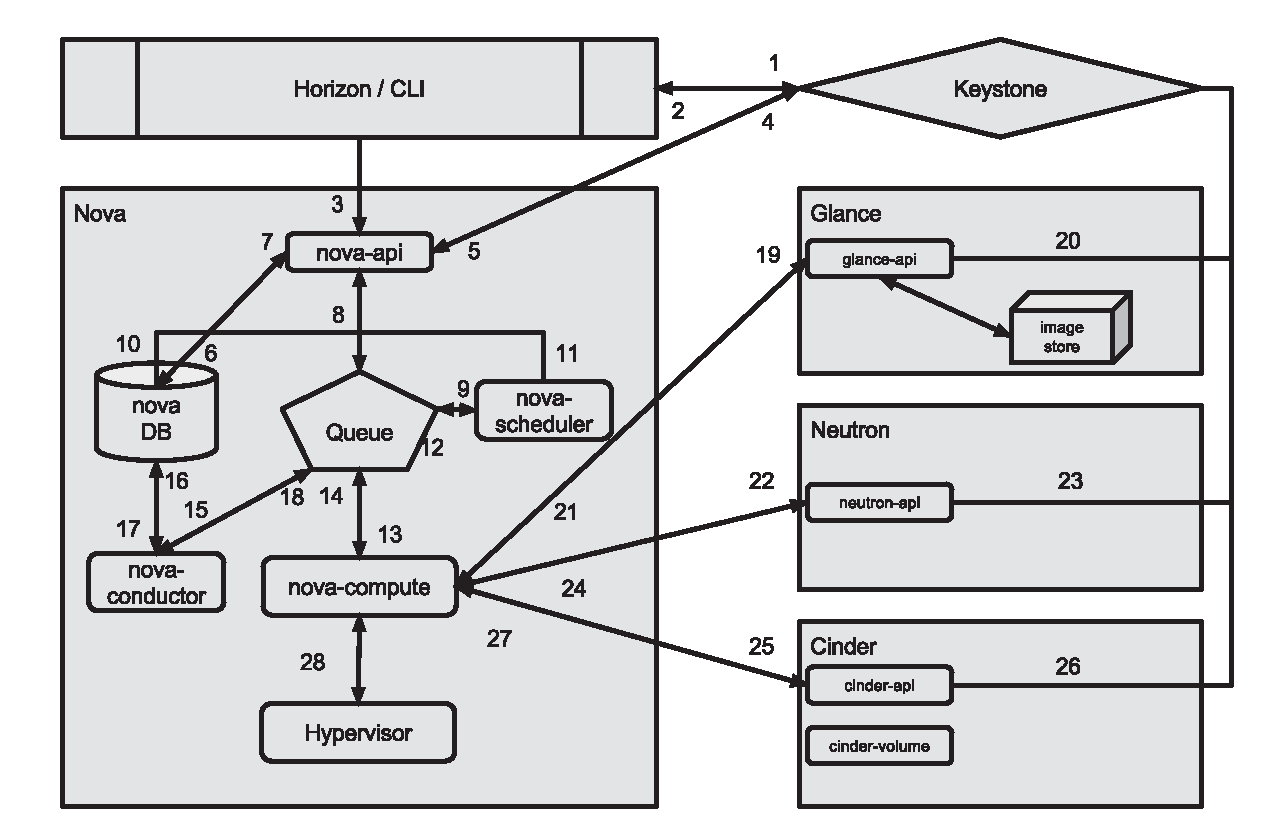
\includegraphics[width=\textwidth]{./img/boot.pdf}
  \end{center}
\end{figure}

\begin{enumerate}
\item \textbf{Horizon or CLI} ユーザの認証情報を取得しRESTの通信によりKeystoneに認証をかけます
\item \textbf{Keystone} ユーザ情報を認証し、認証トークンを生成してユーザにその値を返します。認証トークンは、その他のコンポーネントにREST通信を通してリクエストを投げるためのものです。
\item \textbf{Horizon or CLI Horizon} もしくはCLIは、REST APIにより'launch instance'、もしくは'nova-boot'と定義される新しいインスタンスを生成するリクエストを変換して、それをnova-apiに送ります。
\item \textbf{nova-api} nova-apiは、Keystoneに対してトークンとユーザのパーミッションの確認を行うリクエストを投げます。
\item \textbf{Keystone} Keystoneは、トークンを確認し、更新された認証用ヘッダーをロール情報とパーミッションとともに送ります。
\item \textbf{nova-api} nova-apiはNovaのバックグラウンドのデータベースとのセッションを確立します。
\item \textbf{Database} 新しいインスタンス用のレコードをデータベースに登録します。
\item \textbf{nova-api} nova-apiはnova-schedulerに対してnova-computeのホストIDを決定付けるインスタンスの更新エントリーを除くrpc.callのリクエストを投げます。
\item \textbf{nova-scheduler} nova-schedulerはメッセージングキューを介してリクエストを受けます。
\item \textbf{nova-scheduler} nova-schedulerはNovaのバックエンドのデータベースとセッションを確立し、フィルターと重み付け機能を通してインスタンス生成にふさわしいnova-computeのホストを決定します。
\item \textbf{nova-scheduler} フィルターと重み付け機能を通して決定されたnova-computeのホスト情報を付与したインスタンスのエントリーを返します。
\item \textbf{nova-scheduler} nova-schedulerは、決定されたnova-computeのホストに対して'launch instance'のrpc.castのリクエストを送ります。
\item \textbf{nova-compute} nova-computeはメッセージングキューを介してリクエストを受けます。
\item \textbf{nova-compute} nova-computeはnova-conductorに対してインスタンスのホストのIDやFlavor(メモリ、CPU、ディスク)の情報を取ってくるために、nova-conductorに対してrpc.callのリクエストを投げます。
\item \textbf{nova-conductor} nova-conductorはメッセージングキューを介してリクエストを受けます。
\item \textbf{nova-conductor} nova-conductorはNovaのバックグラウンドのデータベースとのセッションを確立します。
\item \textbf{Database} データベースはインスタンスの情報を返します。
\item \textbf{nova-compute} nova-computeはメッセージングキューを介してリクエストを受けます。
\item \textbf{nova-compute} nova-computeはglance-apiに対して認証トークンを通してブート対象のイメージIDを持ったイメージのURIを取得しイメージ用ストレージからイメージをアップロードするためのRESTのコールを行います。
\item \textbf{glance-api} glance-apiはKeystoneに対して認証トークンを確認しにいきます。
\item \textbf{nova-compute} nova-comupteはイメージのメタデータと取得します。
\item \textbf{nova-compute} nova-computeはNetwork APIに対して認証トークンを通してインスタンスに紐付けるネットワークの割り当てと設定を行うためのRESTのコールを行います。
\item \textbf{neutron-server} neutron-serverはKeystoneに対して認証トークンを確認しにいきます。
\item \textbf{nova-compute} nova-computeはネットワーク情報を取得します。
\item \textbf{nova-compute} nova-computeはVolume APIに対して認証トークンを通してインスタンスにボリュームをアタッチするためのRESTのコールを行います。
\item \textbf{cinder-api} cinder-apiはKeystoneに対して認証トークンを確認しにいきます。
\item \textbf{nova-comupte} nova-computeはブロックストレージの情報を取得します。
\item \textbf{nova-compute} nova-computeはハイパーバイザードライバーのためのデータを生成し、libvirtもしくはAPIを通してハイパーバイザーに対してリクエストを実行します。
\end{enumerate}

以下の表は、上記の各プロビジョニングステップにおけるインスタンスのステータスの変化を表しています。

\begin{table}[htbp]
  \begin{center}
    \begin{tabular}{|l|l|l|l|}
      \hline
      Status & Task & Power state & Steps \\ \hline \hline
      Build & scheduling & None & 3-12 \\ \hline
      Build & networking & None & 22-24 \\ \hline
      Build & block\_device\_mapping & None & 25-27 \\ \hline
      Build & spawing & None & 28 \\ \hline
      Active & none & Running & \\ \hline
    \end{tabular}
  \end{center}
\end{table}

\newpage

\newpage

\chapter{あとがき}

\section*{こじろー}

\subsection*{ミームの死骸を待ちながら}

\begin{quote}
「組織も人も、特殊化の果てにあるのはゆるやかな死、それだけよ」
\end{quote}

\begin{flushright}
草薙素子『GHOST IN THE SHELL / 攻殻機動隊』
\end{flushright}

オープンクラウドという名で、まさに組織が抱えるゆるやかな死を阻止すべく登場したのがOpenStackである。インフラストラクチャーの構築において知の共有がなされていなかった時代、各企業はそれぞれ独自の手法を見出し特殊化していった。2010年代に入り、特殊化が自らのシステムをゆるやかに死に追いやっていることに皆気付き始めた。隔離的に画一化されたシステムは何らかのアクシデントで全滅する可能性がある。考えうる唯一の冴えたやり方は、グローバルな共有知の創出により集団的知性の発生を促すことである。

15年前にGNU/Linuxが成し遂げた夢を、クラウドの分野で再度叶えるのである。この時代にそれを成すためには、ミーム学的アプローチにより、互いに依存しあうミーム複合体(memeplex)を構築することが必要である。偶然か必然か、そのアプローチを取ったのが、OpenStackである。GNU/Linux上に構築されたクラウドシステム(ミーム複合体)とそれと連携するドライバモデル(ミーム)は、まさにミームが寄り集まってミーム複合体を形成する様に酷似しているのである。オープンソースであることはもちろんのこと、単一企業による開発コミュニティの独占が成されていないことにより、共有知の創出を圧倒的速度で促すことに成功したのである。OpenStackによりクラウドのあり方は変わるであろう。が、それと同時に僕は、ミームの死骸に恋い焦がれているのである。

\section*{まっきー}

\subsection*{OpenStackは革命戦士の夢を見るか、あるいはすべてがエスになる世界について}

\begin{quote}
否定性は、止揚の不可欠の一契機である。怒り、等々の否定性の感情は、人が今ある存在を実践的にのりこえ、変換してゆくときに不可欠の前提である。しかしこの怒り、等々の感情は、それがあまりにも直接的で、なまなましくわれわれをおそうとき、われわれの超越への意志を緊縛し、あらがいがたい強力をもって、われわれを内在性のうちにひき戻してしまう。情況にたいしていいったん距離をおき、これを明晰に相対的に把握することを許さない。怒りはわれわれを、情況のたんなる否定性、同位対立者としての境位に呪縛してしまう。(中略)人間的な実践の弁証法は解体し否定性の実存だけがむきだしに残る。そして現代の支配体制の柔構造は、このような無援の実存を愚弄し、吸収するための幾重もの装置をもっている。
\end{quote}

\begin{flushright}
見田宗介『まなざしの地獄』
\end{flushright}

世界を変えるには少なくとも二つの方法がある。一つは、その世界の外に出ること。もう一つは、その世界を変えるだけの地位に付くことだ。かつて集団をもってして世界を変えようとしたかれらに、なぜ我々は手を貸さなかったのか。彼らの臨界点は何だったか。われわれは世界を本当に変えてしまっていいのか。われわれは世界を変えることを望んでいるのか。このあとがきは、主にかつて共に暮らした友人達への謝罪のために書くものである。

その前にOpenStackの話をしよう。OpenStackは確かに良いものであろう。ただ、残念ながらOpenStackで成功を得られるかと言うと、それは何とも答えようがない。まず成功が何かを考えなければならないし、さらに残念なことには、そのようなことは大抵のユーザーにとってはさほど重要なことではない。重要ではないものを話されると何が起きるかというと、時には相手に対する怒りがわくというわけだ。不快だもんね。

革命戦士達に手を貸さなかった理由は、すくなくとも僕にとっては、それが重要ではなかったからだった。重要ではないというのは、重要になるほど不快ではなかったという意味だ。ありていに言えば、別に今の世界に不満はないということだ。従って、僕にとってOpenStackは革命戦士ではない。私は革命を望んではいない。ビッグブラザーは消えたことにしてしまえ。となれば、愛は友人に向けられるべきではないのか。友達が笑っていれば、それでいいのだ。そこはまなざしの地獄かもしれないけれど。

世界の外に出てしまえば、世界を出た自分を認識せねばならない。地位を上るには、地位の高さを自分で認識せねばならない。なるほど是非ともみなやるべきだが、少なくとも僕はやりたくない。それで腹がふくらむわけでもあるまいし。世界の外には無援の実存を愚弄するものも、アブゾーブしてくれる装置もない。だが、世界の中には、両方ある。そこが良い場所だと訓練すれば世界は平和だ。よい場所だと思わせるのが監獄だ。規律と訓練。あぁ、これは語り尽くされたことだった。われわれはそこから出ることは学ばなかったし、出ようとも思わない。

世界をよりよくしたいという思いの居場所を考えないといけないわれわれは、その適用と探索の範囲を、自身にまつわる狭い範疇で認識すればよいものとし、それを世界と呼んだ。見たまえ、やっぱり世界は変わってないじゃないか。君たちのやっていることは迷惑か無意味ではないか。僕は今日も仕事に行く。

時には世の中に違和感を覚え、その解決に行動を起こしたくなる時もあるが、それは僕の生活にとってあまり重要ではなかった。食うに困ったら役所にでも書類を出しにいくか、とか思っている。

得てして、良き友は今でもただの良き友のままであり、僕は革命戦士の夢を見る。怒りがある分には、まだOpenStackもまた、革命戦士の夢をみてもバチはあたらない気がする。

\section*{くろろろろ}

イラスト担当のくろろろろです。人様の原稿に絵を付けたのはこれが初めてなので、とても緊張しました。表紙を見てOpenStackに少しでも興味を持って貰えると嬉しく思います。

\newpage

\begin{flushleft}
\begin{minipage}{0.5\hsize}
\begin{scriptsize}

\subsection*{スタッフプロフィール}

\subsubsection*{本編 こじろーさん}

社会人5 年目の29 才。焦りを感じつつも、メンヘラを誘引する特異体質のため嫁探しは難航を極めている。夜な夜なラブライブのライブBD を泣きながら見ているせいもあると思う。推しはエリチカ(というかむしろナンジョルノ)

\subsubsection*{本編 まっきーさん}

編集長。年齢不詳の社会人3 年目。ツンデレ。大学時代は偏った思想な人と日本一怪しい寮で6 年間を過ごす。コーヒーとお茶のカフェイン漬けな毎日。休日は一歩も外に出たくないしだれとも喋りたくないので社会不適合ギリギリ。自称オタクじゃないけどSHIROBAKO ならみゃーもりになりたい。こじろうさん「この本作ったおかげでコミュ力上がったんじゃね?」

\subsubsection*{絵師様 くろろろろさん}

みさきさん以外をだれも知らないのにイラスト作画を引き受けてくれた天使。ともだちのともだちのともだちはともだち。瀬戸内産のほのぼの絵描きさん。普段癒し系を装うも実はばっさりツッコミ担当。最近はハイキュー及川が尊い。

\subsubsection*{キャラ原案 あおこさん}

(はーと)ラグラージ(はーと)サーナイト(はーと)なべしょ(はーと)しげおか(はーと)年末年始の予定はコミケとルビサファとコンサート。なっぴさん「わたしの愛人も兼ねてますよねグヘヘ」

\subsubsection*{Special Thanks みさきさん}

狩りに出たりイギリスを眺めたりしてると休日が終わる。なんでもおいしくいただける系女子。こじろうさん「ナンジョルノに似てますねフヒヒ」

\subsubsection*{雑用 なっぴさん}

こじろうさんの後輩。このページとキャラプロフィールとキャラ原案と売り子と編集長を急かす担当。セガの作る鏡音レンくんの絶対領域をprprするために可及的速やかに0 と1 に還元されたい。「進捗どうですか、って一回リアルに言ってみたかった。反省はしていない」

\end{scriptsize}
\end{minipage}
\end{flushleft}

\vspace*{\stretch{1}}
\begin{flushright}
\begin{minipage}{0.5\hsize}
\begin{small}
\begin{description}
  \item{制作:} なっぴ
  \item{著者:} こじろう・まっきー
  \item{挿絵:} くろろろろ・あおこ
  \item{初版発行:} 2014年12月30日
  \item{第2版発行:} 2015年12月31日
  \item{印刷:} POPLS (\url{http://www.inv.co.jp/~popls/})
\end{description}
\end{small}
\end{minipage}
\end{flushright}
\vspace*{\stretch{1}}

\newpage

\enlargethispage{\paperwidth}
\thispagestyle{empty}
\vspace*{-1.05truein}
\vspace*{-\topmargin}
\vspace*{-\headheight}
\vspace*{-\headsep}
\vspace*{-\topskip}
\noindent\hspace*{-1.11in}\hspace*{-\oddsidemargin}
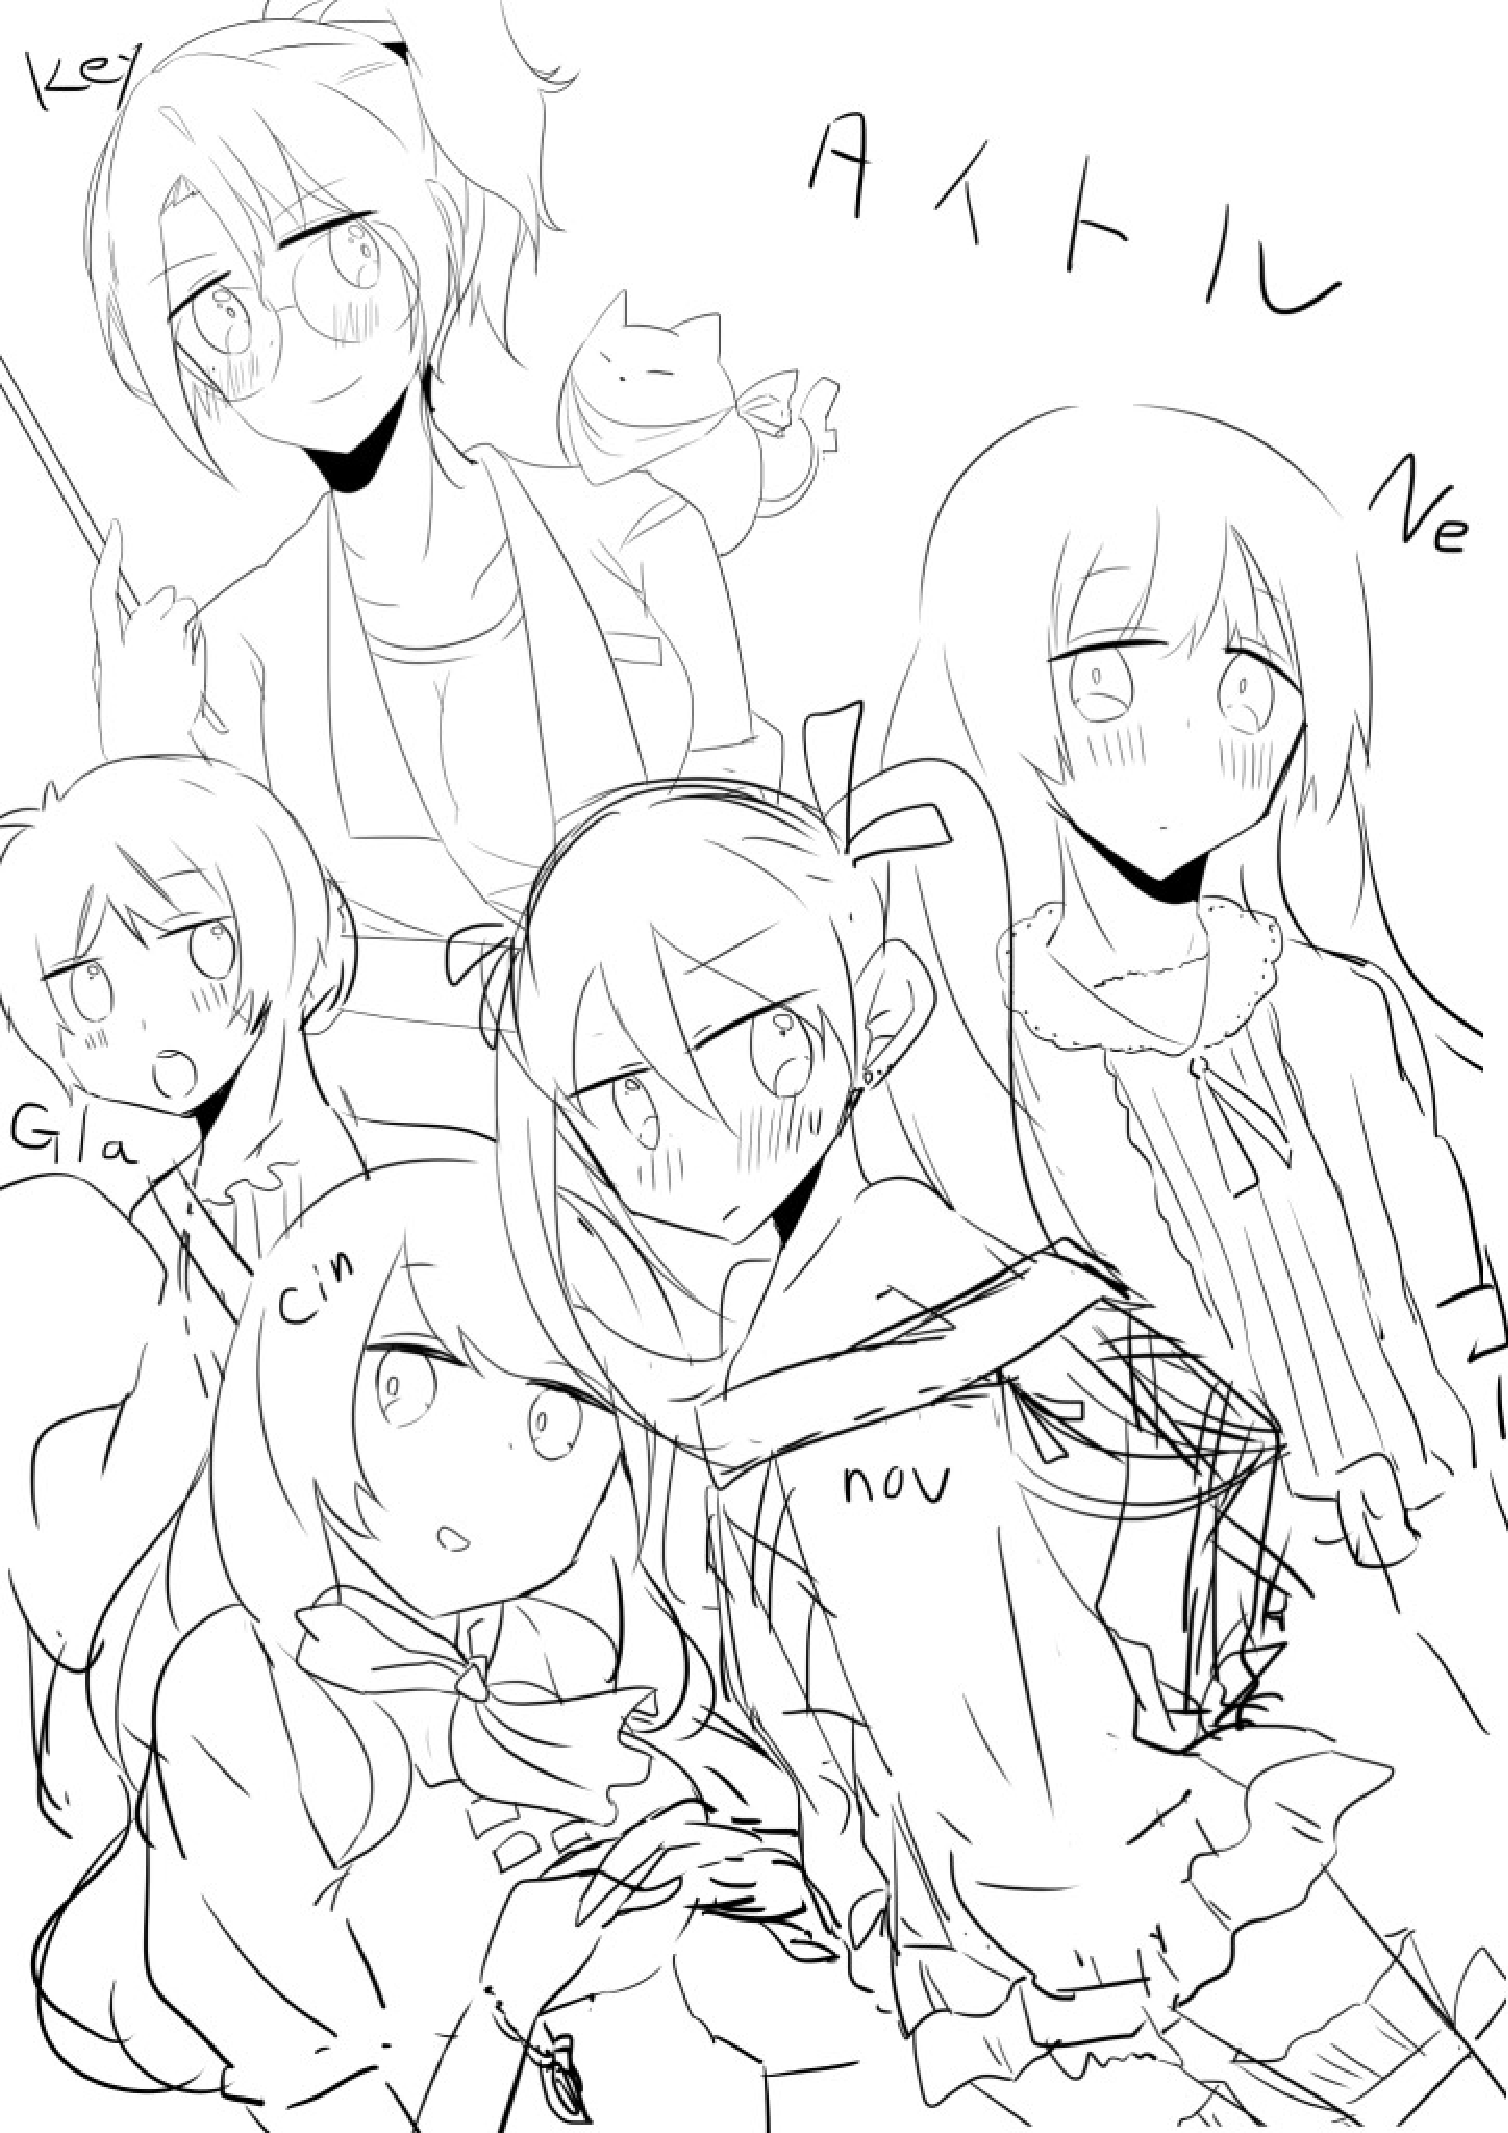
\includegraphics[width=1.025\paperwidth]{./img/bcover.pdf}

\end{document}
